
\section{Multiclass Kernel SVMs}


\subsection{Multiclass SVM strategies}

\subsubsection{spoc-svc}

This method for multi-class classification is based on a new definition of the margin. This generalized notion of margin gives to the method the ability to learn a multi-class classifier simply by solving a constrained optimization
problem with a quadratic objective function.

See \cite{spoc-svc} for more details.


\subsubsection{kbb-svc}

In this case, we extend the binary SVM optimisation problem by adding new decision variables and new constraints. This method implies that the size of the optimisation problem is proportional to the number categories, which can be a problem. 

See \cite{kbb-svc} for more details.


\subsubsection{one-vs-all approach}

The idea is to train one model for each class, that predicts whether a sample belongs to the class or not.
We use KSVM for regression in order to avoid conflicts, which would arise when we would only use binary classification
(i.e. multiple models or no model could predict ``yes'' for the same sample).
Then we can finally predict the class where the model was the most confident (i.e. the regression output is the highest).

\subsubsection{tree-based approach}



\subsection{Parameter optimization and results}

\subsubsection{spoc-svc}

\subsubsection{kbb-svc}

\subsubsection{one-vs-all approach}

We decided to use the RBF-kernel and the same C-parameter for all of the 10 models,
in order to reduce the parameter searchspace.\\
The following plot shows the mean validation accuracy on the ZIP dataset
for different C-parameters, when doing a 10-fold crossvalidation.

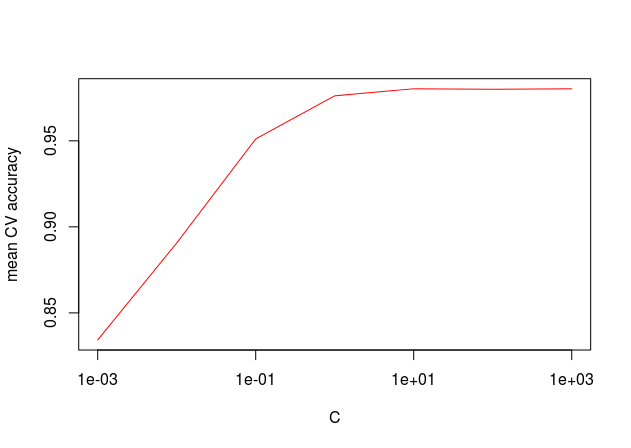
\includegraphics[width=0.8\textwidth]{../plots/one_vs_all_zip}

On the ZIP dataset, the best crossvalidation result was achieved with $C = 1000$,
when comparing 7 different values which were varying from 0.001 to 1000 in a logarithmic scale.\\

Due to a lack of memory and time constraints, we decided to reduce the training set of the MNIST
dataset to 30\% of its original size, which means that 18,000 training images remained.\\
On this new training set the best crossvalidation result was achieved with $C = 100$.\\

With the parameters chosen as described above, we got the following accuracies on the test sets:\\

\begin{tabular}{|c|c|}
 \hline
 dataset[training set size] & test accuracy \\ \hline
 ZIP[7291] & 95.31 \% \\
 MNIST[18000] & 97.97 \% \\
 CIFAR-10[5000] & XX.XX \% \\
 \hline
\end{tabular}


\subsubsection{tree-based approach}